\providecommand{\main}{..}
\documentclass[\main/main.tex]{subfiles}

\begin{document}
\graphicspath{{img/}{ble_mesh/img/}}

\chapter{Bluetooth mesh}

Bluetooth mesh networking provides the foundation to create a truly large-scale device network, allowing tens, hundreds or even thousands of wireless devices to communicate with each other reliably and securely.

Compared with other topologies, in a mesh network, each node may have a direct communication link with many nodes. This brings the robustness to the network against the single point of failure problem but also makes it harder to manage. Figure \ref{fig:Mesh topology} illustrates a basic example of mesh topology.

\begin{figure}[H]
    \begin{center}
        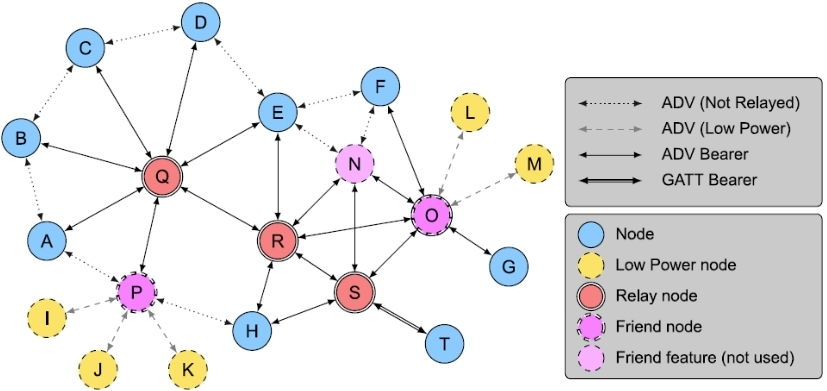
\includegraphics[scale=0.7]{mesh_topology.jpg}
    \end{center}
    \caption{Mesh topology}
    \label{fig:Mesh topology}
\end{figure}


\section{Mesh system architecture \cite{bluetooth_sig:mesh_profile_specification_1_0_1}}
This subsection provides an overview of the mesh network operation and layered system architecture.

\subsection{Layered architecture}

The Mesh Profile specification is defined as a layered architecture as shown in \ref{fig:ble_mesh_layered_architecture}.

\begin{figure}[H]
    \begin{center}
        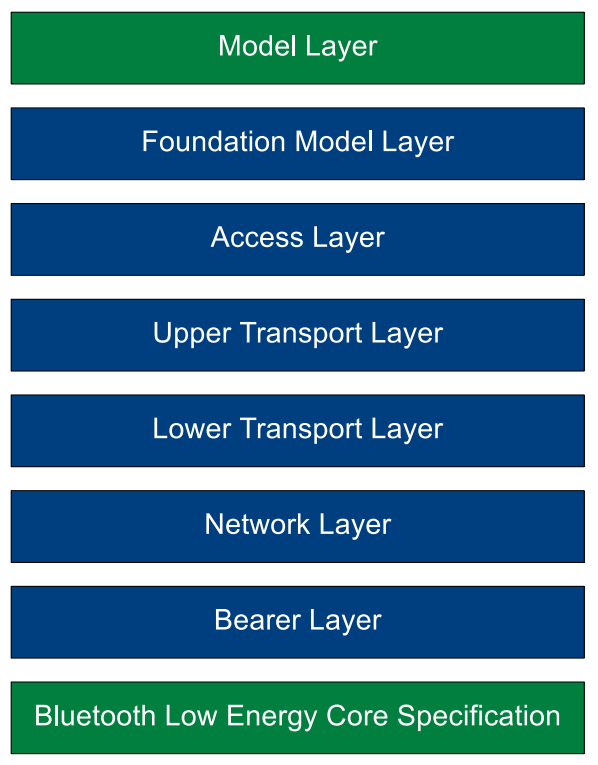
\includegraphics[width=0.4\textwidth]{ble_mesh_layered_architecture.png}
    \end{center}
    \caption{Mesh system architecture}
    \label{fig:ble_mesh_layered_architecture}
\end{figure}

\subsubsection{Model layer}
The Model layer defines models that are used to standardize the operation of typical user scenarios and are defined in the Bluetooth Mesh Model specification or other higher layer specifications. Examples of higher layer model specifications include models for lighting and sensors.

\subsubsection{Foundation Model layer}
The Foundation Model layer defines the states, messages, and models required to configure and manage a mesh network.

\subsubsection{Access layer}
The access layer defines how higher layer applications can use the upper transport layer. It defines the format of the application data; it defines and controls the application data encryption and decryption performed in the upper transport layer; and it checks whether the incoming application data has been received in the context of the right network and application keys before forwarding it to the higher layer

\subsubsection{Upper transport layer}
The upper transport layer encrypts, decrypts, and authenticates application data and is designed to provide confidentiality of access messages. It also defines how transport control messages are used to manage the upper transport layer between nodes, including when used by the Friend feature.

\subsubsection{Lower transport layer}
The lower transport layer defines how upper transport layer messages are segmented and reassembled into multiple Lower Transport PDUs to deliver large upper transport layer messages to other nodes. It also defines a single control message to manage segmentation and reassembly.

\subsubsection{Network layer}
The network layer defines how transport messages are addressed towards one or more elements. It
defines the network message format that allows Transport PDUs to be transported by the bearer layer.
The network layer decides whether to relay/forward messages, accept them for further processing, or
reject them. It also defines how a network message is encrypted and authenticated.

\subsubsection{Bearer layer}
The bearer layer defines how network messages are transported between nodes. There are two bearers
defined, the advertising bearer and the GATT bearer. Additional bearers may be defined in the future.

\subsection{Overview of mesh operation}
The Bluetooth mesh network operation is designed to:
\begin{itemize}
    \item Enable messages to be sent from one element to one or more elements
    \item Allow messages to be relayed via other nodes to extend the range of communication
    \item Secure messages against known security attacks, including eavesdropping attacks, man-in-themiddle attacks, replay attacks, trash-can attacks, brute-force key attacks, and possible additional security attacks not documented here;
    \item Work on existing devices in the market today
    \item Deliver messages in a timely manner
    \item Continue to work when one or more devices are moved or stop operating
    \item Have built-in forward compatibility to support future versions of the Mesh Profile specification
\end{itemize}

Bluetooth mesh is a managed-flood-based network, which uses  broadcast channels to transmit messages so that other nodes can receive messages and relay these messages. Thus extending the range of the original message. Any device in a managed-flood mesh network can send a message at any time. As long as there is a sufficient density of devices that are listening and relaying, messages shall be delivered to the destination. 
\newline\newline
There are a number of methods to restrict the unlimited relaying of messages in a managed-flood mesh network. The two main methods used are the \textbf{network message cache} method and the \textbf{time to live} method.
\newline\newline
The \textbf{network message cache} is designed to prevent devices from relaying previously received messages by adding all messages to a cached list. When a message is received, it is checked against the list and ignored if already present. If not already received, then it is added to the cache so that it can be ignored in the future. To prevent this list from becoming too long, the number of messages that are cached is limited by implementation.
\newline\newline
Each message includes a \textbf{Time to Live} (TTL) value that limits the number of times a message can be relayed. Each time a message is received and then relayed (up to a maximum of 126 times) by a device, the TTL value is decremented by 1.

\subsubsection{Network and subnets}
A mesh network consists of nodes sharing four common resources:
\begin{itemize}
    \item Network addresses used to identify source and destination of messages
    \item Network keys used to secure and authenticate messages at the network layer
    \item Application keys used to secure and authenticate messages at the access layer
    \item An IV Index used to extend the lifetime of the network
\end{itemize}

A network can have one or more subnets that facilitate "area" isolation (e.g., isolated hotel room subnets within a hotel network). A subnet is a group of nodes that can communicate with each other at a network layer because they share a network key. A node may belong to one or more subnets by knowing one or more network keys. At the time of provisioning, a device is provisioned to one subnet and may be added to more subnets using the Configuration Model.
\newline\newline
There is one special subnet called the primary subnet, which is based on the primary NetKey. Nodes on the primary subnet participate in the IV Update procedure, and propagate IV updates to other subnets, while nodes on other subnets only propagate the IV Index updates to those subnets
\newline\newline
The network resources are managed by a node that implements the Configuration Client model, known as the Configuration Client (typically a smartphone or other mobile computing devices) and are allocated to nodes at the time of configuration using the Configuration Server model. In particular, a Provisioner manages allocation of addresses to make sure no duplicate unicast addresses are allocated, whereas a Configuration Client generates and distributes network and application keys and makes sure that devices that need to communicate with each other share proper keys for both network and access layers. The Configuration Client also knows device keys, which are used to secure communication with each individual node, including distributing updated network and application keys.

\subsubsection{Devices and nodes}
A device that is not a member of a mesh network is known as an unprovisioned device. A device that is a member of a mesh network is known as a node. A Provisioner is used to manage the transitions between an unprovisioned device and a node.
\newline\newline
An unprovisioned device cannot send or receive mesh messages; however, it advertises its presence to Provisioners. A Provisioner will invite an unprovisioned device into a mesh network after it has been authenticated, converting the unprovisioned device into a node.
\newline\newline
A node can send or receive mesh messages and is managed by a Configuration Client, that may also be the same device as the Provisioner, over the mesh network to configure how the node communicates with other nodes. A Configuration Client can remove a node from a mesh network, which reverts it back to an unprovisioned device.
\newline\newline
A device may support multiple instances of a node by offering itself to be provisioned to another mesh network after already being provisioned to a mesh network. Each instance of a mesh network is determined by addresses and a device key obtained by the device during provisioning.

\subsubsection{Adding devices to a mesh network}
\textbf{Devices} are added to a mesh network by a Provisioner, at which point they become \textbf{nodes}. The provisioning of devices into a mesh network differs from the point-to-point bonding and pairing that is typically used in Bluetooth wireless technology. Provisioning of devices is enabled using either a simple advertising bearer or a point-to-point GATT-based bearer. A single provisioning protocol is used over both bearers. Provisioning over an advertising-based bearer is implemented by all devices. Provisioning over a GATT-based bearer allows devices such as legacy phones (i.e., devices that do not support provisioning over an advertising bearer natively) to be Provisioners.
\newline\newline
To assist with \textbf{provisioning of multiple devices}, a device has an attention timer that can be set by a Provisioner. When set to a non-zero value, the device \textbf{identifies itself} using any means it can. For example, the device may flash a light, make a sound, or vibrate. When the attention timer expires, the device stops identifying itself. This allows a Provisioner to send a single message to a device to cause it to identify itself and the device automatically stops identifying itself after a given time.
\newline\newline
The protocol to run over these two bearers is a derivative of the Security Manager protocol of v4.2 of the Bluetooth Core Specification to introduce the ability to authenticate devices that have a very limited user interface, such as a light or a switch. The Security Manager protocol requires a reliable bearer, something that cannot be guaranteed by the advertising provisioning bearer; therefore the protocol is designed to enable reliable delivery of messages independent of the bearer. The similarity to the Security Manager protocol enables significant reuse of existing code on devices that have implemented such functionality.

\subsection{Architectural concepts}
The Bluetooth mesh networking architecture uses several different concepts: states, messages, elements, addressing, models, publish-subscribe, mesh keys, etc.
\subsubsection{States}
A state is a value representing a condition of an element.
\newline\newline
An element exposing a state is referred to as a server. For example, the simplest server is a Generic OnOff Server, representing that it is either on or off.
\newline\newline
An element accessing a state is referred to as a client. For example, the simplest client is a Generic OnOff Client (a binary switch) that is able to control a Generic OnOff Server via messages defined by the Generic OnOff Model.
\newline\newline
States that are composed of two of more values are known as composite states. For example, a color-changing lamp can control color hue separately from color saturation and brightness.
\subsubsection{Messages}
All communication within a mesh network is accomplished by sending messages. Messages operate on states. For each state, there is a defined set of messages that a server supports and a client may use to request a value of a state or to change a state. A server may also transmit unsolicited messages carrying information about states and/or changing states.
\newline\newline
A message is defined as having an opcode, associated parameters, and behavior. An opcode may be a single octet (for special messages that require maximum possible payload for parameters), 2 octets (for standard messages), or 3 octets (for vendor-specific messages).
\newline\newline
A total message size, including an opcode, is determined by the underlying transport layer, which may use a Segmentation and Reassembly (SAR) mechanism. To maximize performance and avoid the overhead of SAR, a design goal is to fit messages in a single segment. The transport layer provides up to \textbf{11 octets} for a non-segmented message, leaving up to \textbf{10 octets} that are available for parameters when using a \textbf{1-octet opcode}, up to \textbf{9 octets} available for parameters when using a \textbf{2-octet opcode}, and up to \textbf{8 octets} available for parameters when using a vendor-specific \textbf{3-octet opcode}.
\newline\newline
The transport layer provides a mechanism of SAR capable of transporting up to 32 segments. The maximum message size when using the SAR is 384 octets. This means (excluding an Application MIC) up to 379 octets are available for parameters when using a 1-octet opcode, up to 378 octets are available for parameters when using a 2-octet opcode, and up to 377 octets are available for parameters when using a vendor-specific 3-octet opcode
\newline\newline
SAR effectively does not impose any extra overhead on the access layer payload per segment: a 10-octet message is transported as an unsegmented message, and a 20-octet message is transported as a segmented message that uses two segments.
\newline\newline
Message definitions contain tables of parameters. In a message payload, parameters follow an opcode, and parameter offsets are in octets unless otherwise specified.
\newline\newline
Messages are defined as acknowledged or unacknowledged. An acknowledged message requires a response whereas an unacknowledged message does not require a response

\subsubsection{Elements}
An element is an addressable entity within a node. \textbf{Each node has at least one element, the primary element, and may have one or more additional secondary elements}. The number and structure of elements is static and does not change throughout the lifetime of a node (that is, as long as the node is part of a network).
\newline\newline
The primary element is addressed using the first unicast address assigned to the node during provisioning. Each additional secondary element is addressed using the subsequent addresses. These unicast element addresses allow nodes to identify which element within a node is transmitting or receiving a message.
\newline\newline
If the number and structure of elements changes, for example due to a firmware update, the node must be re-provisioned. The Node Removal procedure is used when a firmware update is performed that changes the number or structure of elements.
\newline\newline
Messages are dispatched within models based on opcodes and element addresses.
\newline\newline
An element is not allowed to contain multiple instances of models that use the same message in the same way (for example, receive an “On” message). When multiple models within the same element use the same message, the models are said to “overlap.” To implement multiple instances of overlapping models within a single node (for example, to control multiple light fixtures that can be turned on and off), the node is required to contain multiple elements.
\newline\newline
For example, a light fixture may have two lamps, each implementing an instance of the Light Lightness Server model and an instance of the Generic Power OnOff Server model. This requires that the node contain two elements, one for each lamp. When it receives an "On" message, the node uses the unicast
address of the element to identify which instance of the Generic Power OnOff Server model the message is addressed to.
\newline\newline
In another example, a dual-socket power strip contains two independent energy measurement sensors that can measure power consumed by an appliance connected to a socket. This would require that the node have two Sensor Data states, each in a separate element. The first element, the primary element,
would be identified using the unicast address for the node and would include a state for the first energy sensor as well as states representing the configuration of the node. The second element, a secondary element, would be identified using a unicast element address and would include the state for the second energy sensor.
\newline\newline
Each element has a GATT Bluetooth Namespace Descriptor value that helps identify which part of the node this element represents. These namespace descriptor values use the same definitions as GATT. For example, the elements of the temperature sensor would use the values “inside” and “outside".

\subsubsection{Addresses}
An address may be a unicast address, a virtual address, or a group address. There is also a special value to represent an unassigned address that is not used in messages.
\newline\newline
A \textbf{unicast address} is allocated to an element and always represents a single element of a node. There are 32767 unicast addresses per mesh network.
\newline\newline
A \textbf{virtual address} is a multicast address and can represent multiple elements on one or more nodes. Each virtual address logically represents a Label UUID, which is a 128-bit value that does not have to be managed centrally. Each message sent to a Label UUID includes the full Label UUID in the message integrity check value that is used to authenticate the message. To reduce the overhead of checking every known Label UUID, a hash of the Label UUID is used. There are 16384 hash values, each of which codifies a set of virtual addresses. While there are only 16384 hash values used in a virtual address, each hash value can represent millions of possible Label UUIDs; therefore, the number of virtual addresses is considered very large.
\newline\newline
A \textbf{group address} is a multicast address and can represent multiple elements on one or more nodes. There are 16384 group addresses per mesh network. There are a set of fixed group addresses that are used to address a subset of all primary elements of nodes based on the functionality of those nodes. All other group addresses are known as dynamically assigned group addresses. There are 256 fixed group addresses and 16128 dynamically assigned group addresses.
\subsubsection{Models}
\textbf{A model defines the basic functionality of a element. A element may include multiple models}. A model defines the required states, the messages that act upon those states, and any associated behavior. 
\newline\newline
A mesh application is specified using a client-server architecture communicating with a publish-subscribe paradigm. Due to the nature of mesh networks and the recognition that the configuration of behavior is performed by a Configuration Client, an application is not defined in a single end-to-end specification such as a profile. Instead, an application is defined in a client model, a server model, and a control model.
\newline\newline
There are three types of model: server models, client models, and control models:
\begin{itemize}
    \item \textbf{Server model}: A server model is composed of one or more states spanning one or more elements. The server model defines a set of mandatory messages that it can transmit or receive, the behavior required of the element when it transmits and receives such messages, and any additional behavior that occurs after messages are transmitted or received.
    \item \textbf{Client model}: A client model defines a set of messages (both mandatory and optional) that a client uses to request, change, or consume corresponding server states, as defined by a server model. The client model does not have state.
    \item \textbf{Control model}: A control model may contain client model functionality to communicate with other server models and server model functionality to communicate with other client models. A control model may also contain control logic, which is a set of rules and behaviors that coordinate the interactions between other models that the control model connects to.
\end{itemize}
A single device may include server, client, and control models.
\subsubsection{Publish-subscribe and message exchange}
Publication and subscription of data within the mesh network is described as using a publish-subscribe paradigm. Nodes that generate messages publish the messages to a unicast address, group address, or virtual address. Nodes that are interested in receiving the messages will subscribe to these addresses.
\newline\newline
Generated messages are sent to destination mesh addresses that can be unicast, pre-configured group addresses, or virtual addresses. Messages can be sent as replies to other messages or can be unsolicited messages. When an instance of a model is sending a reply message, it uses the incoming message originator’s source address as the destination address. When an instance of a model is sending unsolicited messages, it uses a model publish address as the destination address. Each instance of a model within a node has a single publish address.
\newline\newline
On the receiving side, each instance of a model within a node can subscribe to one or more group addresses or virtual addresses. Whenever a message that is addressed to a group address or a virtual address on one of the model’s subscription lists arrives, it is processed by the node. A message is also processed when its destination address is the unicast address of a receiving element or when its destination address is a fixed group address that this device is a member of. If a node has multiple elements, then the message is processed once on each of the addressed elements.
\newline\newline
Publish addresses and subscription lists for models defined by higher layer specifications use the Model Publication and Subscription List states that are managed by the Configuration Server Model.
\newline\newline
A node can have multiple subscriptions per instance of a model’s element, although nodes may limit the number of subscriptions that are supported. Using multiple subscription addresses allows a node to respond to messages that are published to different groups. For example, a light may be subscribed to messages sent to the bedside light group, the bedroom group, the upstairs group, and the house group.
\newline\newline
Each message is sent from a single unicast address (an element address) and sequenced using a unique sequence number to facilitate detection of and protection against replay attacks.

\subsubsection{Security}
All messages are encrypted and authenticated using two types of keys. One key type is for the network layer communication, such that all communication within a mesh network would use the same network key. The other key type is for application data. Separating the keys for networking and applications allows sensitive access messages (e.g., for access control to a building) to be separated from non-sensitive access messages (e.g., for lighting). There are no unencrypted or unauthenticated messages within a mesh network.
\newline\newline
\textbf{Application and network security}: Encrypting and authenticating messages at the upper transport layer and network layer is designed to secure communications within the mesh network against eavesdroppers and malicious attacks. Each layer maintains distinct keys to allow separation between application and network entities.
\newline\newline
\textbf{Obfuscation}: The network security model utilizes a privacy mechanism called obfuscation that utilizes AES to encrypt the source address, sequence numbers, and other header information using a privacy key. The intent for obfuscation is to make tracking nodes more difficult.
\newline\newline
\textbf{Network and application key identifiers}: A node may have multiple network or application keys. By using a key identifier, it is possible to identify which subset of keys are used to secure the message. For example, instead of checking 20 keys, a node may only need to check two keys that have the same least significant bits of the key identifier. If a message is received with a key identifier that is not known, then the node can immediately discard it. The key identifier is generated from the network or application key using a key derivation function.
\newline\newline
\textbf{Initialization vector index}: A Network PDU contains a 24-bit sequence number that allows an element to transmit 16,777,216 Network PDUs. The sequence number is used in the security nonce to provide uniqueness; therefore the sequence number must not wrap. If an element is transmitting a new message at 2 Hz, then these sequence numbers would be exhausted after 97 days. To enable a mesh network to operate for longer periods of time than the sequence number space allows, an additional 4-octet value called the IV Index is defined that is included in the security nonce. For example, using the same 2 Hz message frequency would measure the lifetime of the network using the IV Index in billions of years.

\section{Bluetooth mesh-based application with NimBLE}
\label{sec:bluetooth_mesh_based_application_with_nimble}
Apache NimBLE is an open-source Bluetooth 5.1 stack (both Host and Controller) that completely replaces the proprietary SoftDevice on Nordic chipsets. It is part of the Apache Mynewt project \cite{web_nimble}.

The following are some highlighted features of NimBLE:
\begin{itemize}
    \item Support for 251-byte packet size
    \item Support for all 4 roles concurrently - Broadcaster, Observer, Peripheral and Central
    \item Support for up to 32 simultaneous connections
    \item Legacy and SC (secure connections) SMP support (pairing and bonding)
    \item Advertising extensions is available
    \item Coded (aka Long Range) and 2M PHYs
    \item Bluetooth Mesh supported
\end{itemize}

This subsection introduces the process of defining a Bluetooth mesh-based application with NimBLE which includes 3 steps:
\begin{itemize}
    \item Define a node
    \item Define elements in the node
    \item Define models in each element
    \item Define model operations in each model
\end{itemize}
\subsection{Node composition}
As discussed in previous sections, a node may consist of one or more elements. In NimBLE, a node is defined by a struct as shown in figure \ref{fig:node_struct}. The thee upper components is the ID of the node itself:
\begin{itemize}
    \item CID: Company ID
    \item VID: Vendor ID
    \item PID: Product ID
\end{itemize}
The $elem$ component is a pointer to an array of elements with  size of $elem\_count$.

\begin{figure}[H]
    \begin{lstlisting}[style=CStyle]
struct bt_mesh_comp {
	u16_t cid;
	u16_t pid;
	u16_t vid;

	size_t elem_count;
	struct bt_mesh_elem *elem;
};
    \end{lstlisting}
    \caption{Node struct}
    \label{fig:node_struct}
\end{figure}

Figure \ref{fig:node_struct_example} is an example for defining a node with $g\_elements$ array. The definition for  $g\_elements$ will be provided subsequently.
\begin{figure}[H]
    \begin{lstlisting}[style=CStyle]
static const struct bt_mesh_comp g_comp = {
    .cid = 0x05C3,
    .elem = g_elements,
    .elem_count = ARRAY_SIZE(g_elements)
};
    \end{lstlisting}
    \caption{Node struct example}
    \label{fig:node_struct_example}
\end{figure}

\subsection{Mesh element}
Figure \ref{fig:mesh_element} illustrates the definition of the mesh element. Each elements of a node have a 16-bit unique address in the network $addr$. Moreover, a element may have one or more models as the theory introduced. These models of the element are pointed by the two lower components: $models$ and $vnd\_models$ (vendor model). Figure \ref{fig:mesh_element_example} provides the definition for $g\_elements$ array of the node. As shown if figure \ref{fig:mesh_element_macro}, a macro is used to define an element. The second parameter of the function-like macro ($model\_root$) is a pointer to an array of models. The definition for  $model\_root$ will be provided subsequently.
\begin{figure}[H]
    \begin{lstlisting}[style=CStyle]
struct bt_mesh_elem {
    /* Unicast Address. Set at runtime during provisioning. */
    u16_t addr;

    /* Location Descriptor (GATT Bluetooth Namespace Descriptors) */
    const u16_t loc;

    const u8_t model_count;
    const u8_t vnd_model_count;

    struct bt_mesh_model * const models;
    struct bt_mesh_model * const vnd_models;
};
    \end{lstlisting}
    \caption{Mesh element}
    \label{fig:mesh_element}
\end{figure}

\begin{figure}[H]
    \begin{lstlisting}[style=CStyle]
static struct bt_mesh_elem g_elements[] = {
    BT_MESH_ELEM(0, model_root, BT_MESH_MODEL_NONE),
};
    \end{lstlisting}
    \caption{Mesh element example}
    \label{fig:mesh_element_example}
\end{figure}

\begin{figure}[H]
    \begin{lstlisting}[style=CStyle]
#define BT_MESH_ELEM(_loc, _mods, _vnd_mods)        \
{                                                   \
    .loc              = (_loc),                 \
    .model_count      = ARRAY_SIZE(_mods),      \
    .models           = (_mods),                \
    .vnd_model_count  = ARRAY_SIZE(_vnd_mods),  \
    .vnd_models       = (_vnd_mods),            \
}
    \end{lstlisting}
    \caption{Mesh element macro}
    \label{fig:mesh_element_macro}
\end{figure}

\subsection{Mesh model}
The definition for the mesh model is given in figure \ref{fig:mesh_model}. The following are explanation for important fields:
\begin{itemize}
    \item $elem\_idx$: the index of the element to which the model belong
    \item  $model\_idx$: the index of the model inside the element.
    \item $pub$: the special object initialized in the provisioning process, used to send messages to an address.
    \item $keys$: an array of application key used for this model to communicate.
    \item $groups$: an array of subscribed addresses. They are group or virtual addresses because the unicast address has been already saved in the element. When a received message arrives to the access layer, the model will check if the message destination address is equal to element's unicast address or an address in the $groups$ array for further processing.
    \item $op$: an array of operations defined for this model.
\end{itemize}
Figure \ref{fig:mesh_model_example} shows the definition of $model\_root$. A definition for configuration server is provided in figure \ref{fig:mesh_configuration_server}. As given in figure \ref{fig:mesh_model_macro}, an model is define using a function-like macro. The third parameter $model\_pub\_rtls$ is a static object passed to the macro without any initialization. The second parameter $rtls\_op$ and its definition will be introduce subsequently.
\begin{figure}[H]
    \begin{lstlisting}[style=CStyle]
struct bt_mesh_model {
    union {
        const u16_t id;
        struct {
            u16_t company;
            u16_t id;
        } vnd;
    };

    /* Internal information, mainly for persistent storage */
    u8_t  elem_idx;   /* Belongs to Nth element */
    u8_t  mod_idx;    /* Is the Nth model in the element */
    u16_t flags;      /* Information about what has changed */

    /* Model Publication */
    struct bt_mesh_model_pub * const pub;

    /* AppKey List */
    u16_t keys[CONFIG_BT_MESH_MODEL_KEY_COUNT];

    /* Subscription List (group or virtual addresses) */
    u16_t groups[CONFIG_BT_MESH_MODEL_GROUP_COUNT];

    const struct bt_mesh_model_op * const op;

    /* Model-specific user data */
    void *user_data;
};
    \end{lstlisting}
    \caption{Mesh model}
    \label{fig:mesh_model}
\end{figure}

\begin{figure}[H]
    \begin{lstlisting}[style=CStyle]
struct bt_mesh_model model_root[] = {
    BT_MESH_MODEL_CFG_SRV(&cfg_srv),
    BT_MESH_MODEL(BT_MESH_MODEL_ID_RTLS, rtls_op, &model_pub_rtls, NULL),
};
    \end{lstlisting}
    \caption{Mesh model example}
    \label{fig:mesh_model_example}
\end{figure}

\begin{figure}[H]
    \begin{lstlisting}[style=CStyle]
#define BT_MESH_MODEL(_id, _op, _pub, _user_data)                            \
{                                                                            \
	.id = (_id),                                                         \
	.op = _op,                                                           \
	.keys = { [0 ... (CONFIG_BT_MESH_MODEL_KEY_COUNT - 1)] =             \
			BT_MESH_KEY_UNUSED },                                \
	.pub = _pub,                                                         \
	.groups = { [0 ... (CONFIG_BT_MESH_MODEL_GROUP_COUNT - 1)] =         \
			BT_MESH_ADDR_UNASSIGNED },                           \
	.user_data = _user_data,                                             \
}
\end{lstlisting}
\caption{Mesh model macro}
\label{fig:mesh_model_macro}
\end{figure}

\begin{figure}[H]
    \begin{lstlisting}[style=CStyle]
static struct bt_mesh_cfg_srv cfg_srv = {
    .relay = BT_MESH_RELAY_DISABLED,
    .beacon = BT_MESH_BEACON_ENABLED,
    .frnd = BT_MESH_FRIEND_NOT_SUPPORTED,
    .gatt_proxy = BT_MESH_GATT_PROXY_ENABLED,
    .default_ttl = 7,
    .net_transmit = BT_MESH_TRANSMIT(0, 10),
    .relay_retransmit = BT_MESH_TRANSMIT(0, 10),
};
\end{lstlisting}
\caption{Mesh configuration server}
\label{fig:mesh_configuration_server}
\end{figure}

\subsection{Mesh operation}
The struct of the mesh operation is given in figure \ref{fig:mesh_model_operation}. The two main components of the struct are the operation code $opcode$ and the function handler called when receiving a message with operation code $opcode$. Figure \ref{fig:mesh_model_operation_example} provide the definition for $rtls\_op$. After checking for the destination address, the access layer will check for the operation code of the message, if the callback handler is available for that $opcode$, such function will be called.

\begin{figure}[H]
    \begin{lstlisting}[style=CStyle]
struct bt_mesh_model_op {
	/* OpCode encoded using the BT_MESH_MODEL_OP_* macros */
	const u32_t  opcode;

	/* Minimum required message length */
	const size_t min_len;

	/* Message handler for the opcode */
	void (*const func)(struct bt_mesh_model *model,
			   struct bt_mesh_msg_ctx *ctx,
			   struct os_mbuf *buf);
};
    \end{lstlisting}
    \caption{Mesh operation}
    \label{fig:mesh_model_operation}
\end{figure}

\begin{figure}[H]
    \begin{lstlisting}[style=CStyle]
static const struct bt_mesh_model_op rtls_op[] = {
    { BT_MESH_MODEL_OP_SET, 0, rtls_model_set},
    BT_MESH_MODEL_OP_END,
};
\end{lstlisting}
\caption{Mesh operation example}
\label{fig:mesh_model_operation_example}
\end{figure}

\section{Using Bluetooth mesh for best-effort broadcast service}
\label{sec:using_bluetooth_mesh_for_best_effort_broadcast_service}
In this thesis, all nodes subscribe and publish to a group address which is 0xC000. Anchors and tags subscribe to the SET operation and publish STATUS operation while gateways subscribe to STATUS operation and publish SET operation. This makes a SET message from a gateway broadcasted to all tags and anchors in the network and a STATUS message from an anchor or tag shall be transmitted to a gateway. Figure \ref{fig:ble_mesh_comunication} illustrates the idea of broadcast service over a publish-subscribe paradigm. Since the message sent to a group address is not acknowledged, the service provided by the network is the best-effort service. This means that there is no guarantee that the packet will be delivered to the final destination. 

\begin{figure}[H]
    \begin{center}
        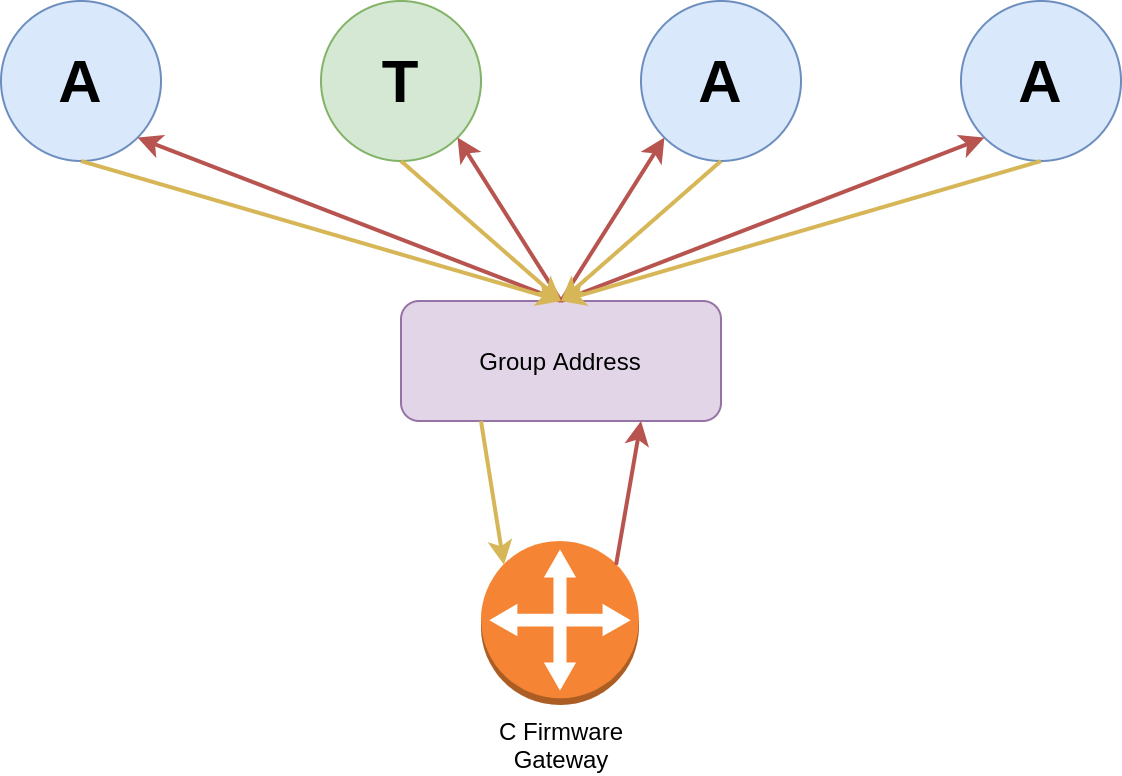
\includegraphics[width=0.7\textwidth]{ble_mesh_comunication.png}
    \end{center}
    \caption{ble mesh communication}
    \label{fig:ble_mesh_comunication}
\end{figure}

In section \ref{sec:bluetooth_mesh_based_application_with_nimble}, the process of defining a Bluetooth mesh-based device has been introduced. In the next section, an Android application manipulated to make such devices communicate as discussed in this section will be described.
\section{nRF Mesh Android application}
The nRF Mesh application is a provisioner making an unprovisioned device become a node in the Bluetooth mesh network. 

Figure \ref{fig:bluetooth_mesh_device_scan} shows that there is one mesh capable device around the provisioner. The address of the device in the network after being provisioned is configured as shown in figure \ref{fig:config_device_address}. This is the address of the primary element, all other elements of the node are addressed by increasing this value by 1 after each element.

\begin{figure}[H]
    \centering
    \begin{subfigure}[b]{0.4\linewidth}
        \centering
        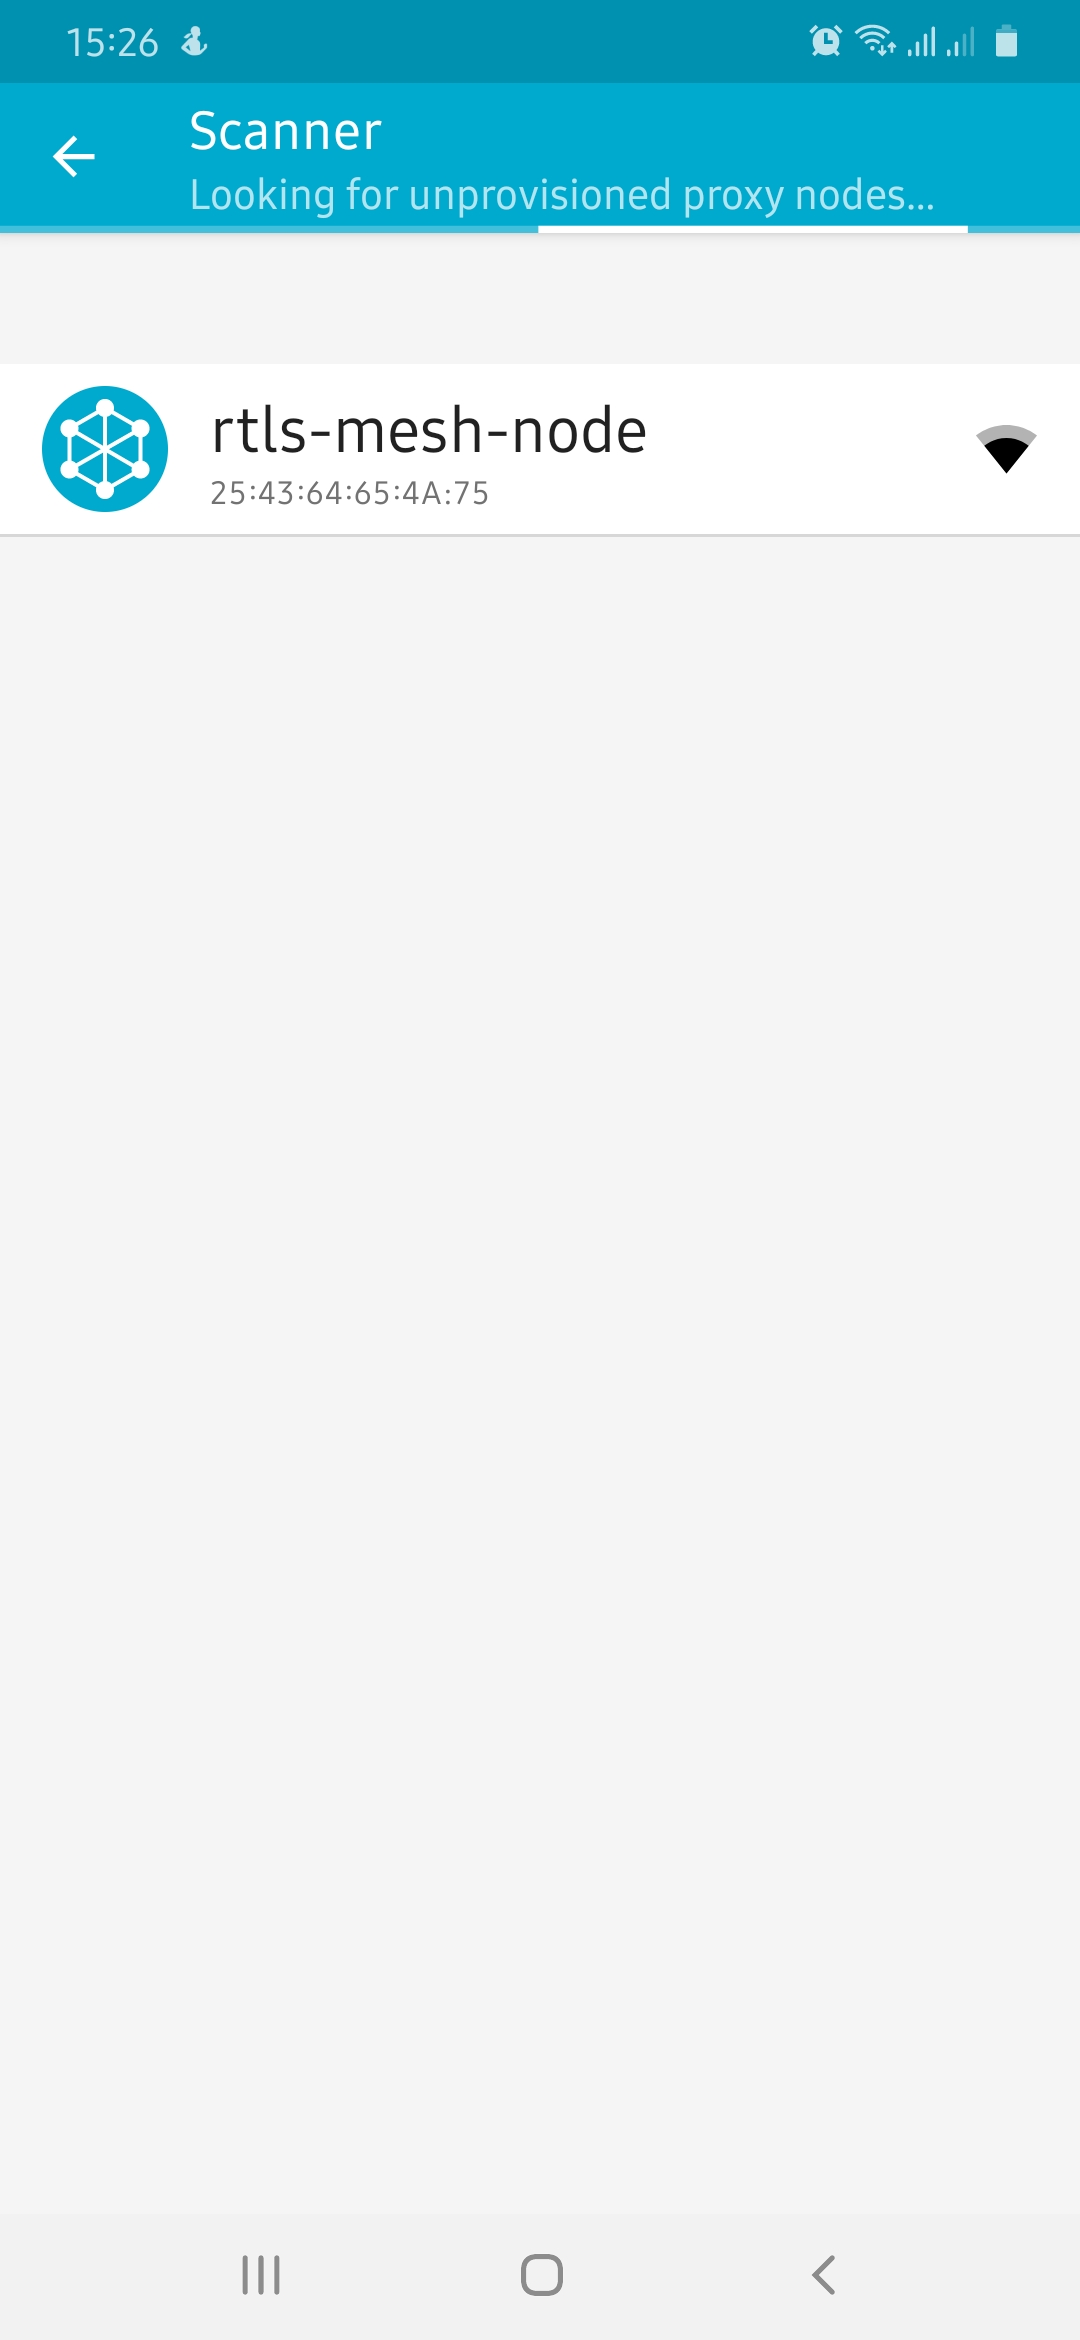
\includegraphics[width=0.7\linewidth]{nRF_Mesh_00.jpg}
        \caption{Bluetooth mesh device scan}
        \label{fig:bluetooth_mesh_device_scan}
    \end{subfigure}
    \begin{subfigure}[b]{0.4\linewidth}
        \centering
        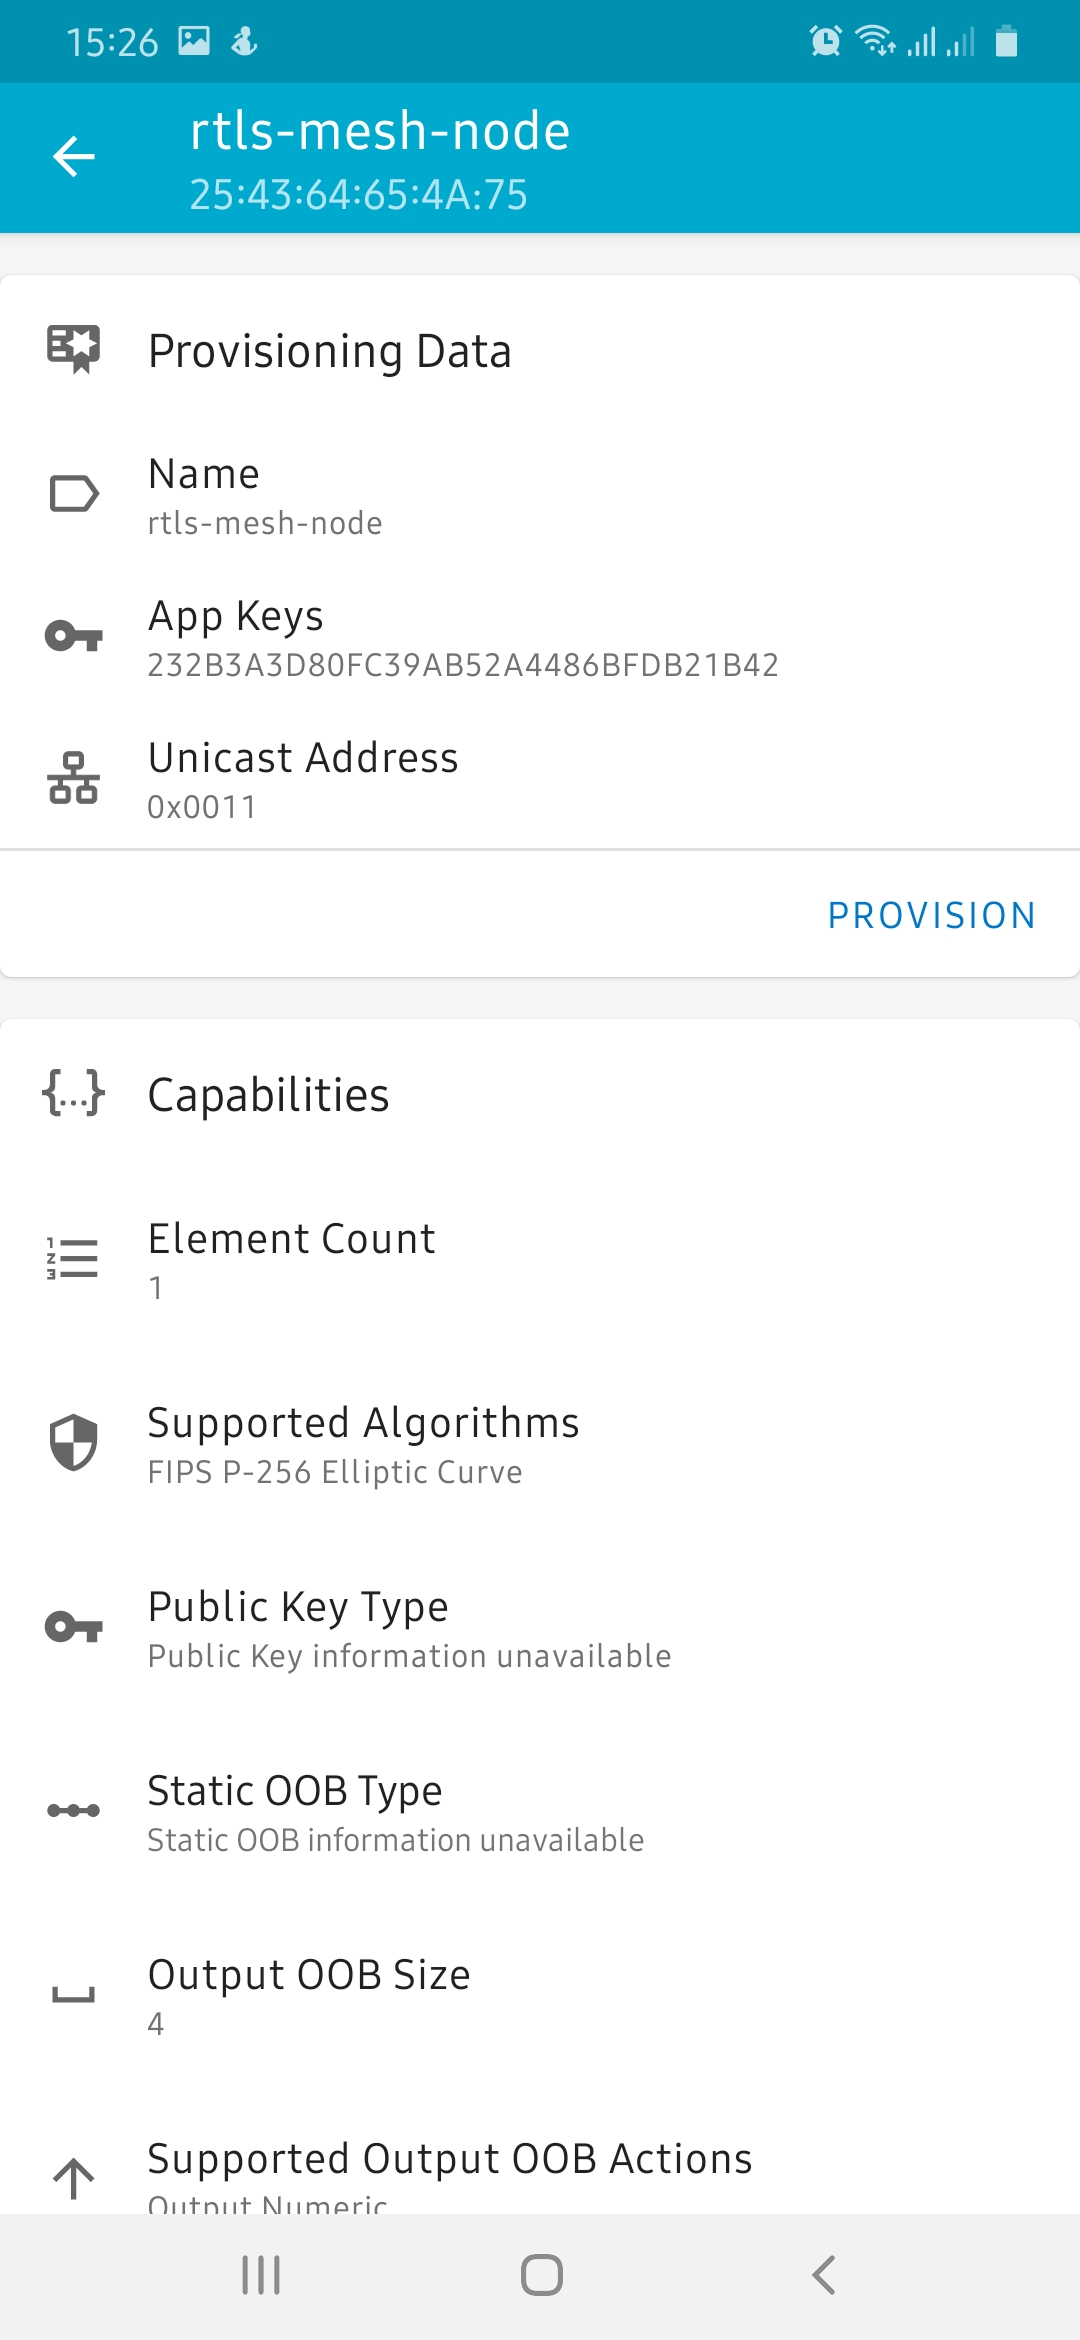
\includegraphics[width=0.7\linewidth]{nRF_Mesh_01.jpg}
        \caption{Config device address}
        \label{fig:config_device_address}
    \end{subfigure}
    \caption{Device provision with nRF Mesh}
    \label{fig:device_provision_with_nrf_mesh_00}
\end{figure}

Figure \ref{fig:device_provision_with_nrf_mesh_01} illustrates the provisioning process done automatically by the Android app and the mesh-capable device.

After a device is successfully provision, a new node appears in the node list as shown in figure \ref{fig:bluetooth_mesh_node_list}. As given in figure \ref{fig:node_element}, the provisioner finds that the node has only one element consisting of two models. The model which has the ID 0x1000 is the custom model built in section \ref{sec:bluetooth_mesh_based_application_with_nimble}. 

The final step is to assign an application key, publish and subscribe address for the model as illustrated in figure \ref{fig:element_configuration}. The publish and subscribe address is 0xC000 as discussed in section \ref{sec:using_bluetooth_mesh_for_best_effort_broadcast_service}.

\begin{figure}[H]
    \centering
    \begin{subfigure}[b]{0.4\linewidth}
        \centering
        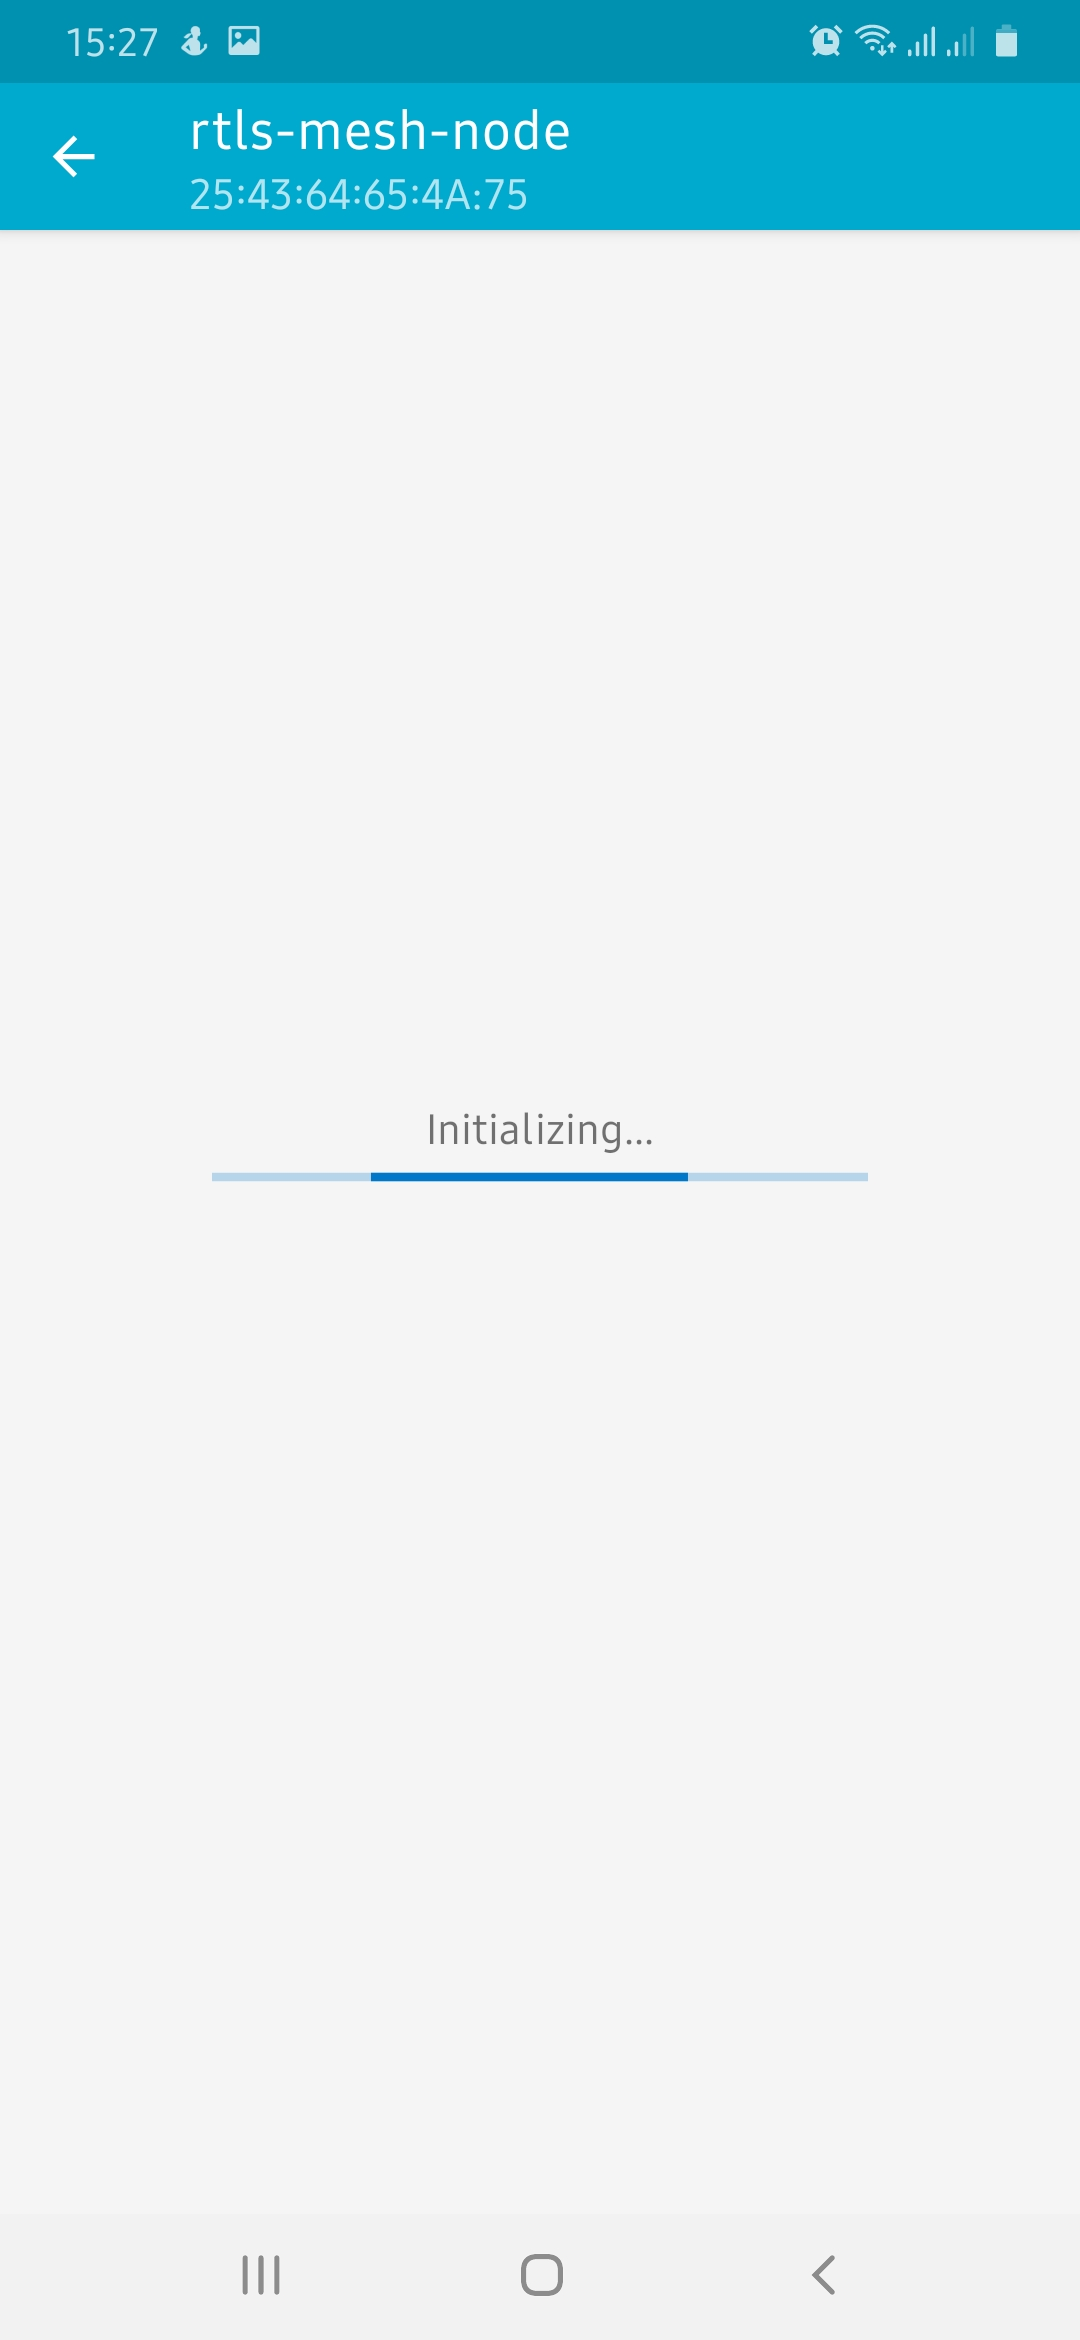
\includegraphics[width=0.65\linewidth]{nRF_Mesh_02.jpg}
        \caption{Bluetooth mesh provisioning}
    \end{subfigure}
    \begin{subfigure}[b]{0.4\linewidth}
        \centering
        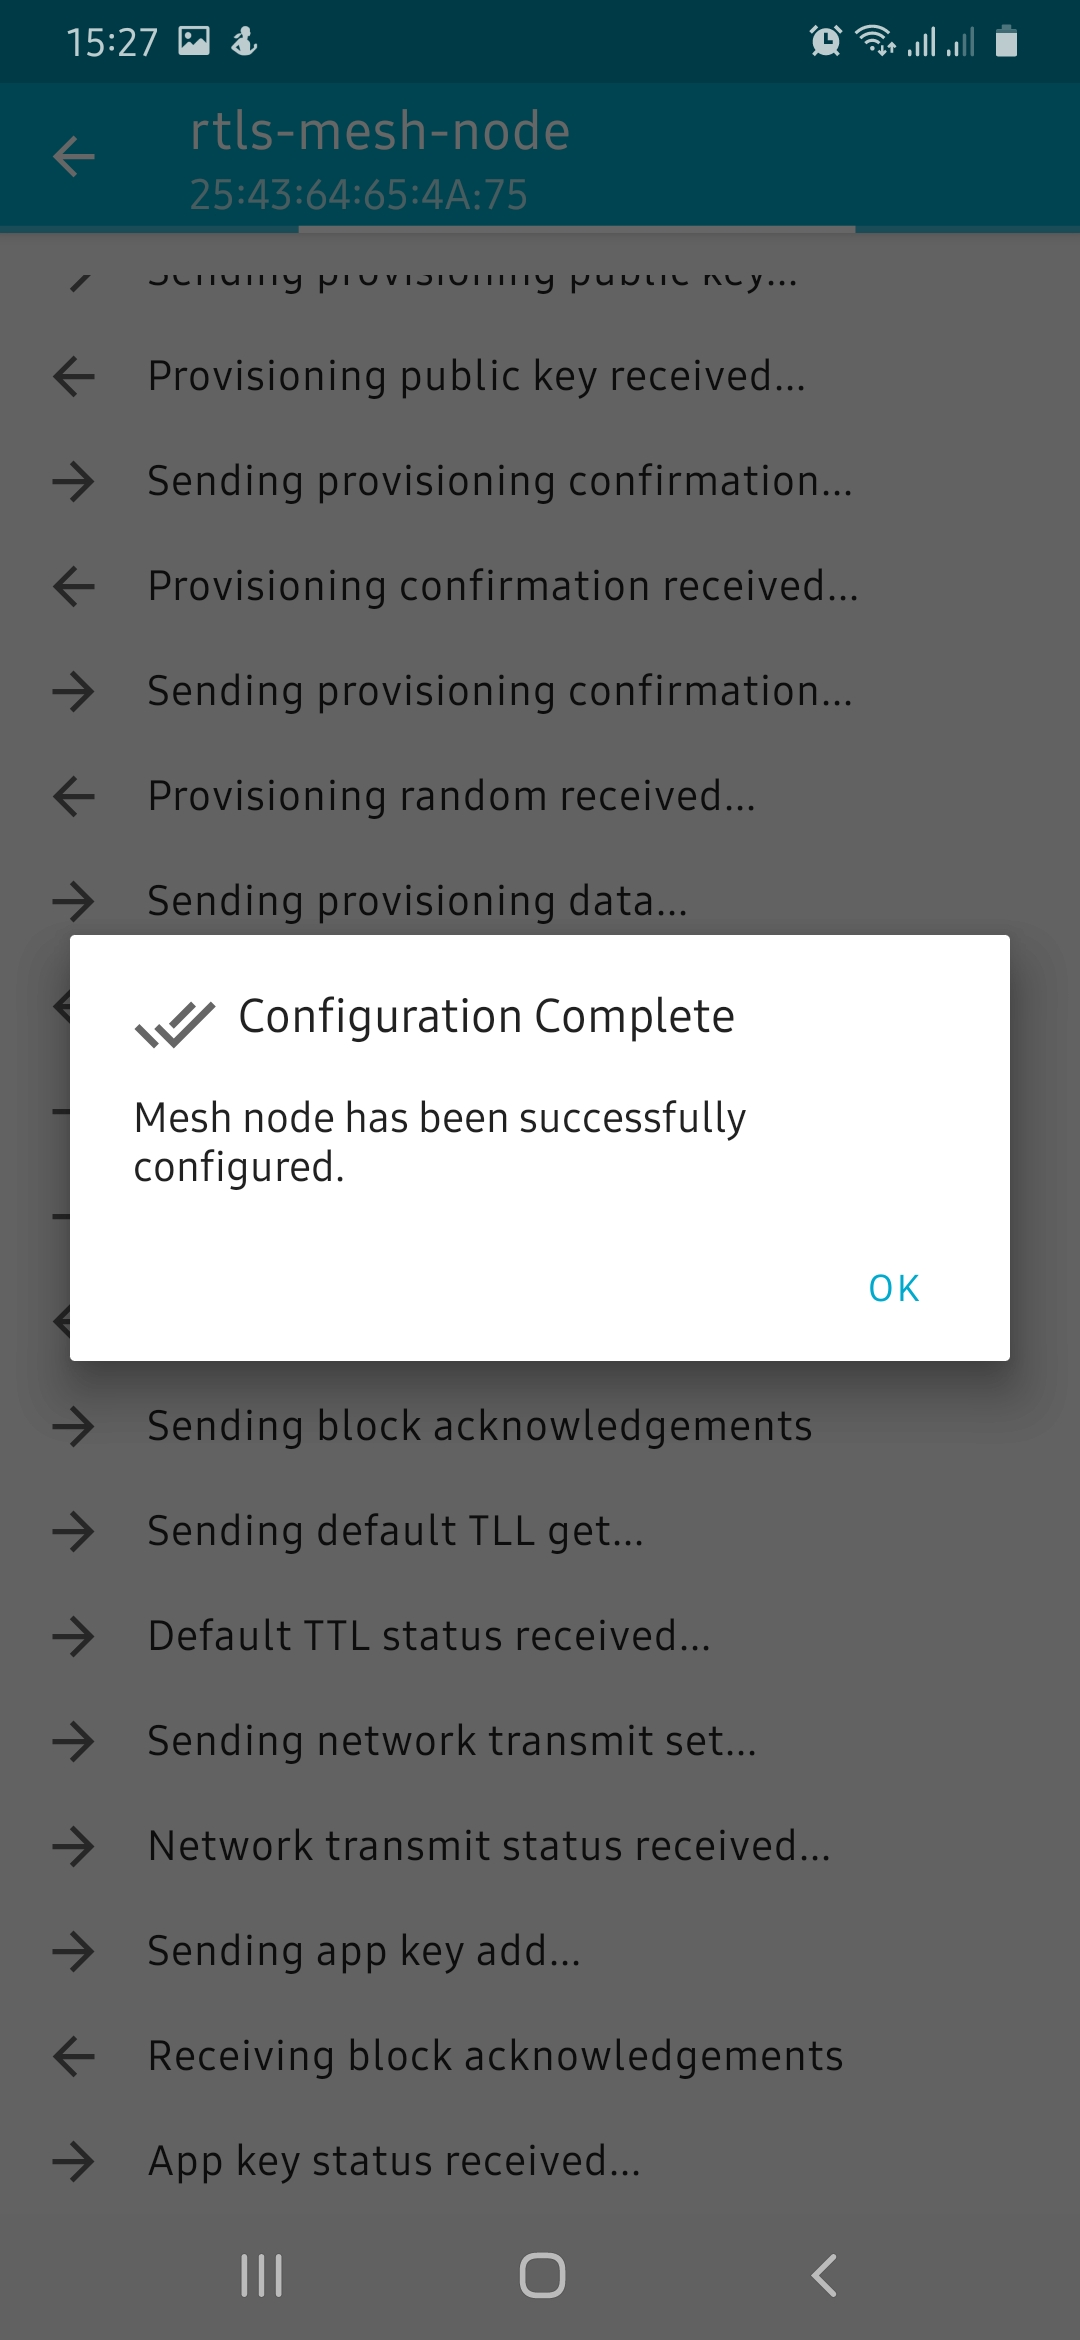
\includegraphics[width=0.65\linewidth]{nRF_Mesh_03.jpg}
        \caption{Device provision complete}
    \end{subfigure}
    \caption{Device provision with nRF Mesh}
    \label{fig:device_provision_with_nrf_mesh_01}
\end{figure}

\begin{figure}[H]
    \centering
    \begin{subfigure}[b]{0.4\linewidth}
        \centering
        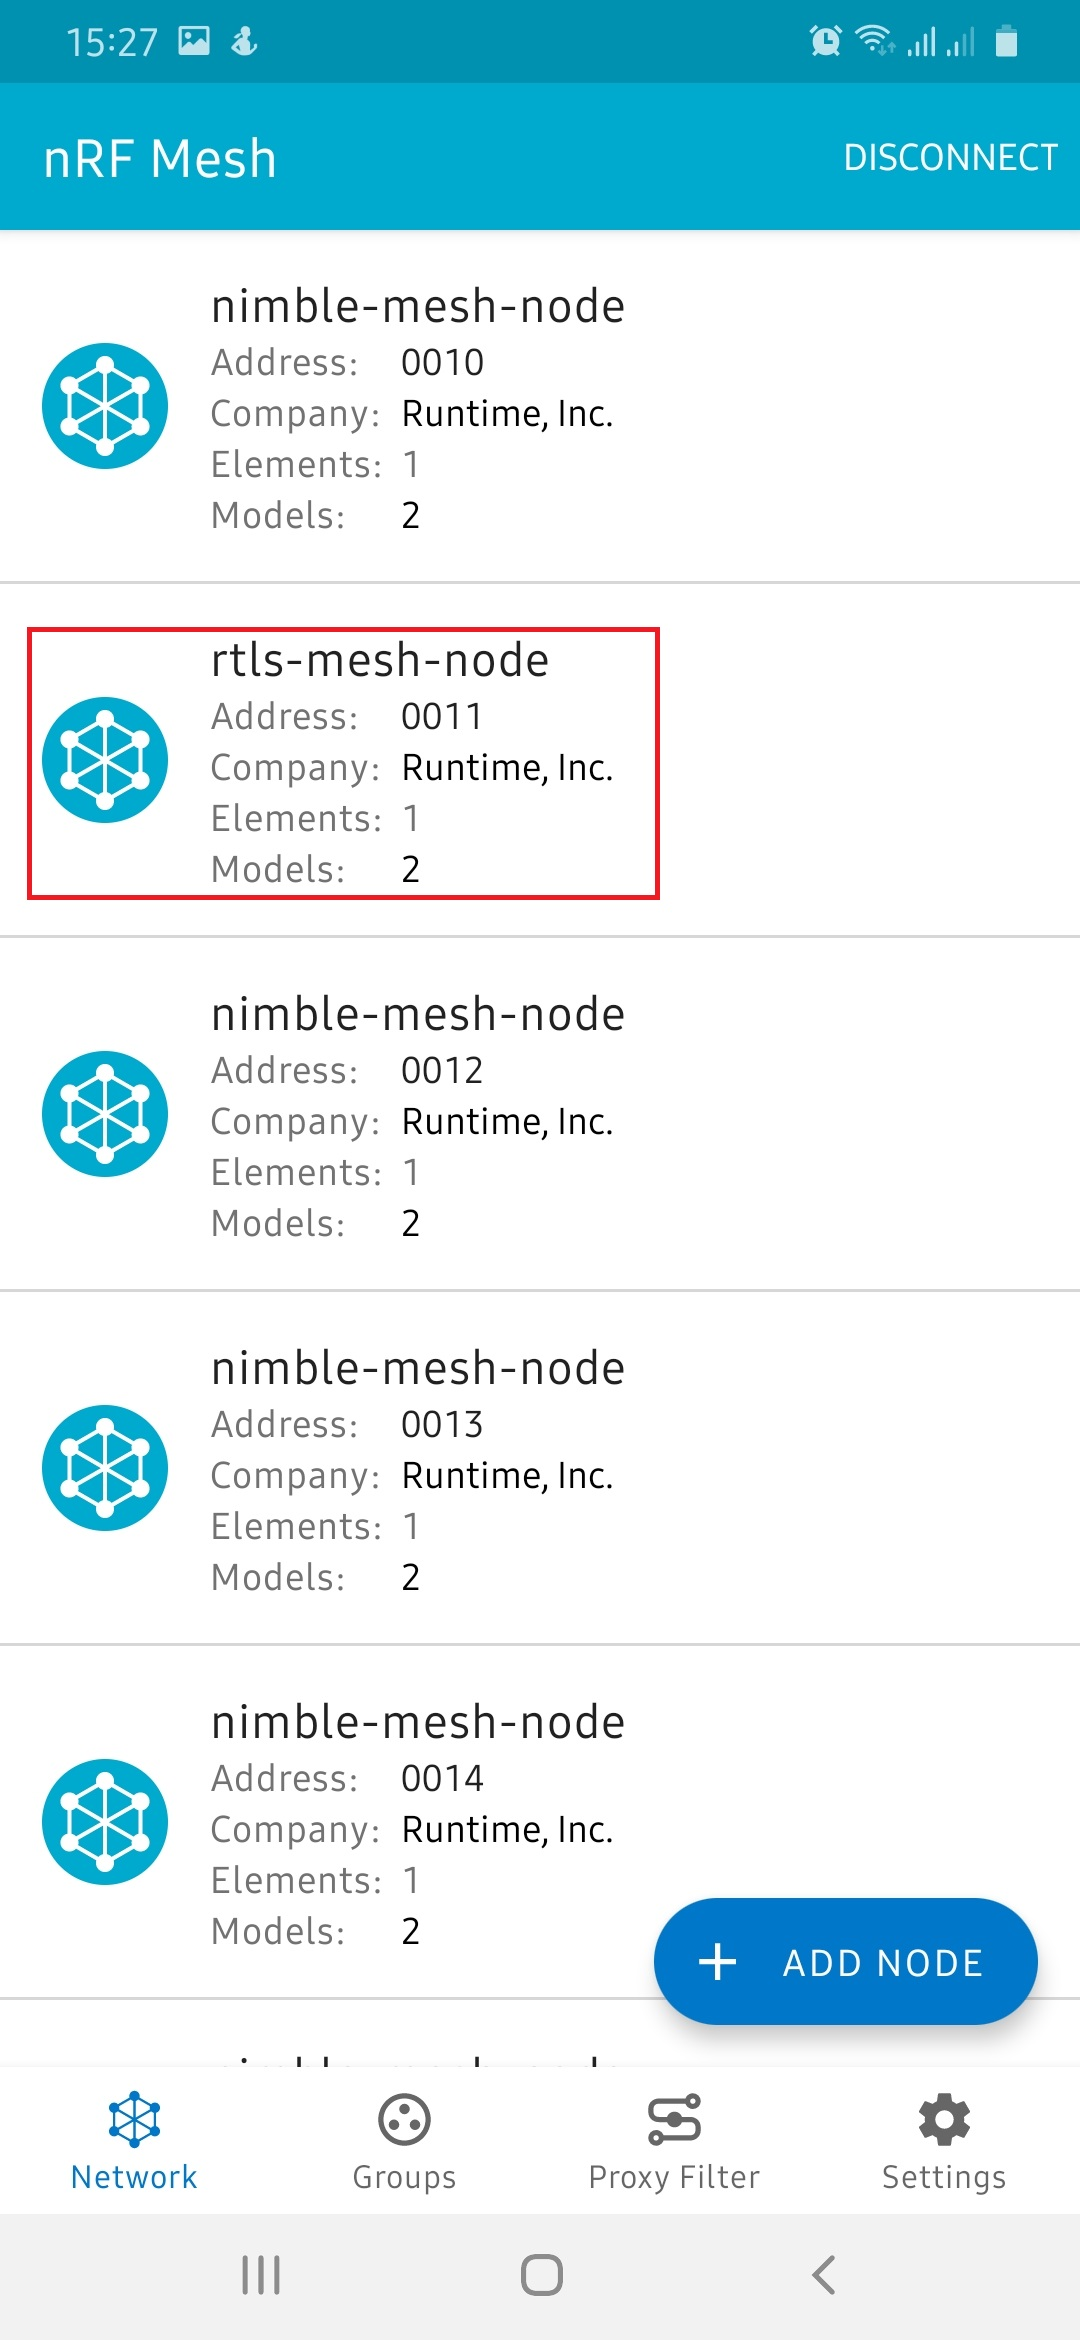
\includegraphics[width=0.65\linewidth]{nRF_Mesh_04.jpg}
        \caption{Bluetooth mesh node list}
        \label{fig:bluetooth_mesh_node_list}
    \end{subfigure}
    \begin{subfigure}[b]{0.4\linewidth}
        \centering
        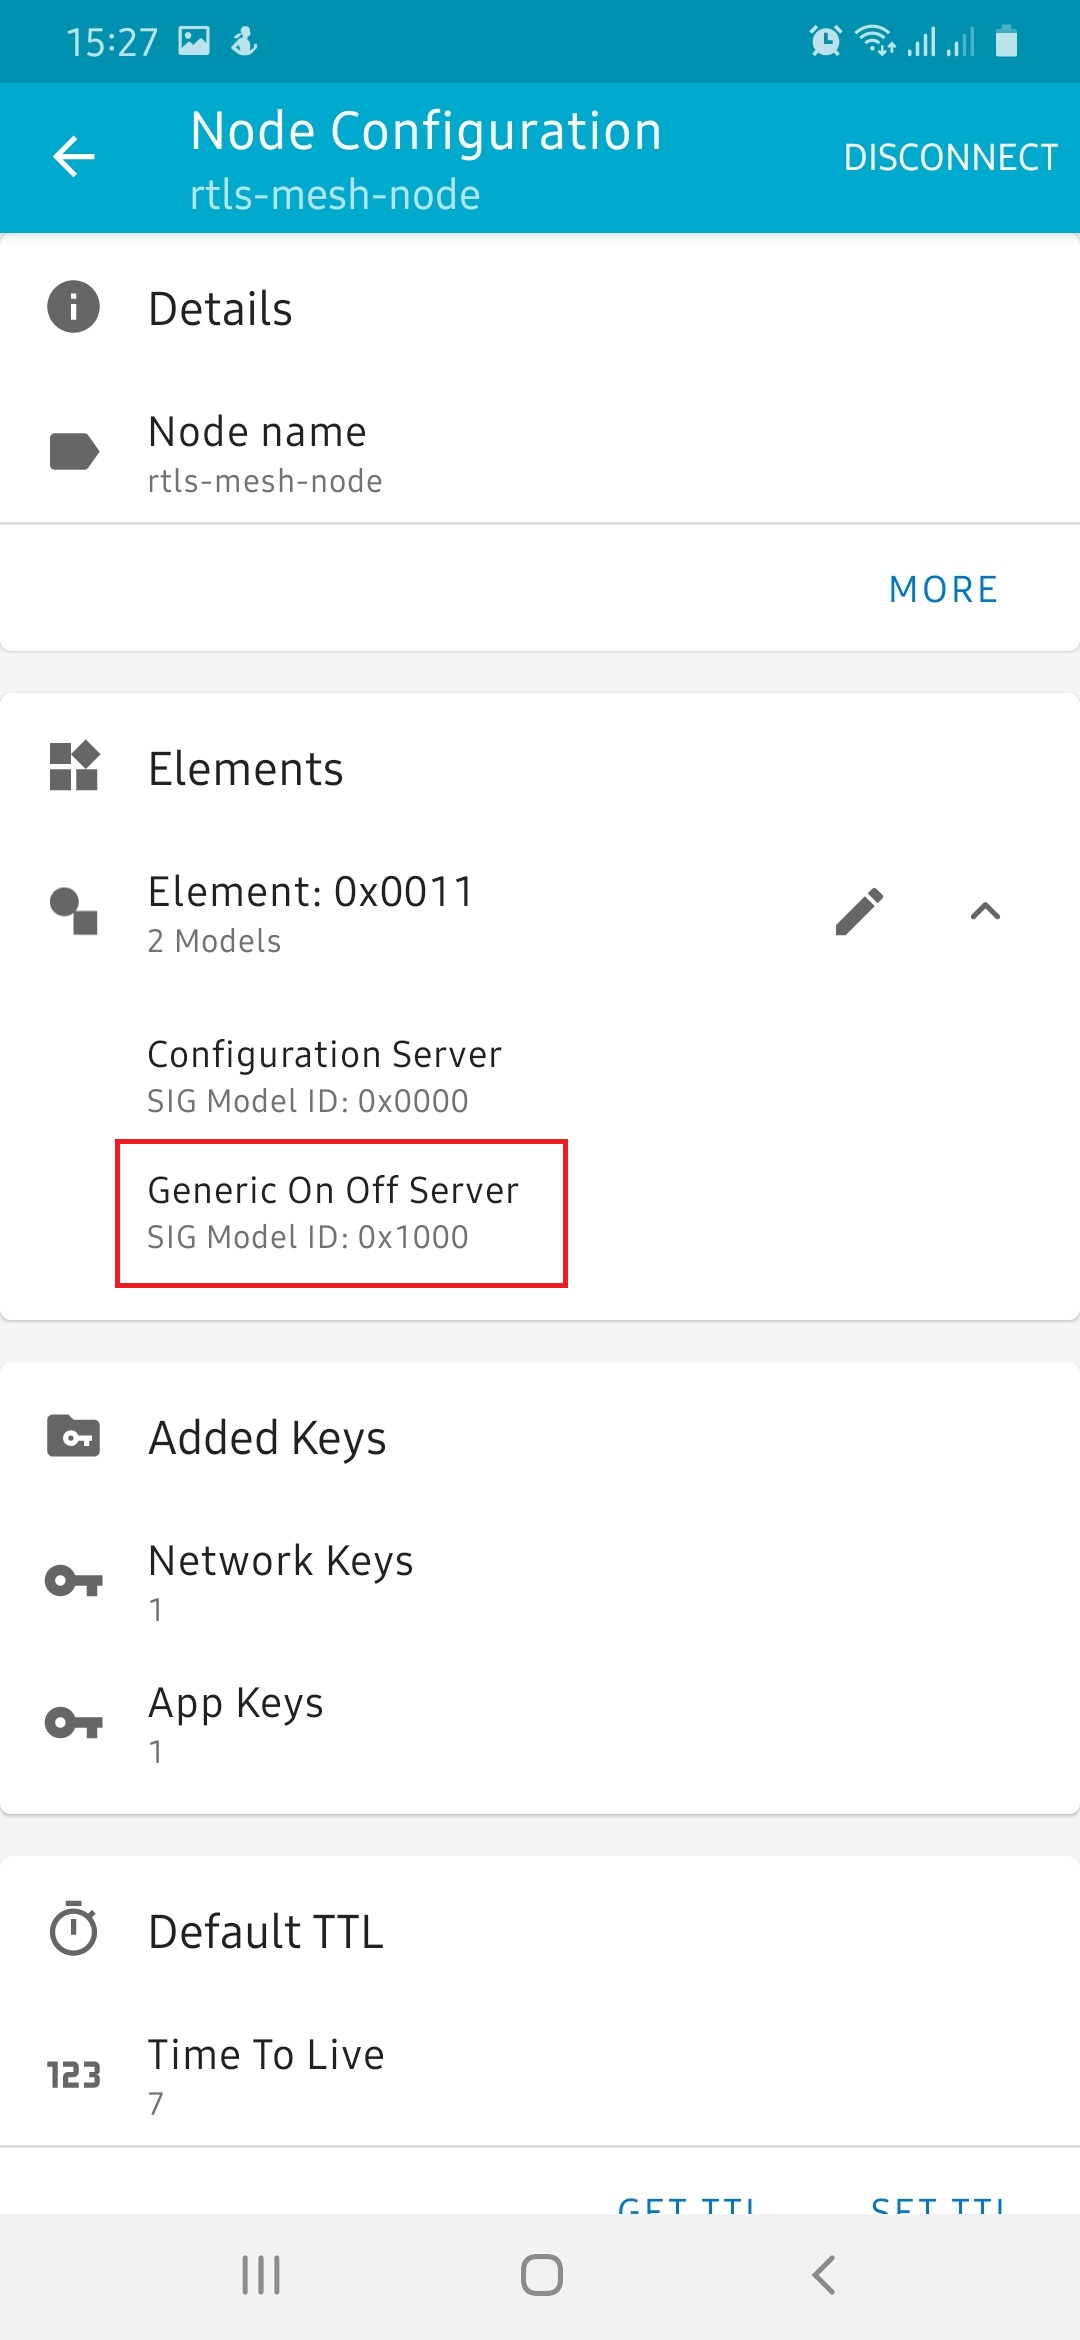
\includegraphics[width=0.65\linewidth]{nRF_Mesh_05.jpg}
        \caption{Node information tab}
        \label{fig:node_element}
    \end{subfigure}
    \caption{Node information}
    \label{fig:node_information}
\end{figure}

\begin{figure}[H]
    \centering
    \begin{subfigure}[b]{0.4\linewidth}
        \centering
        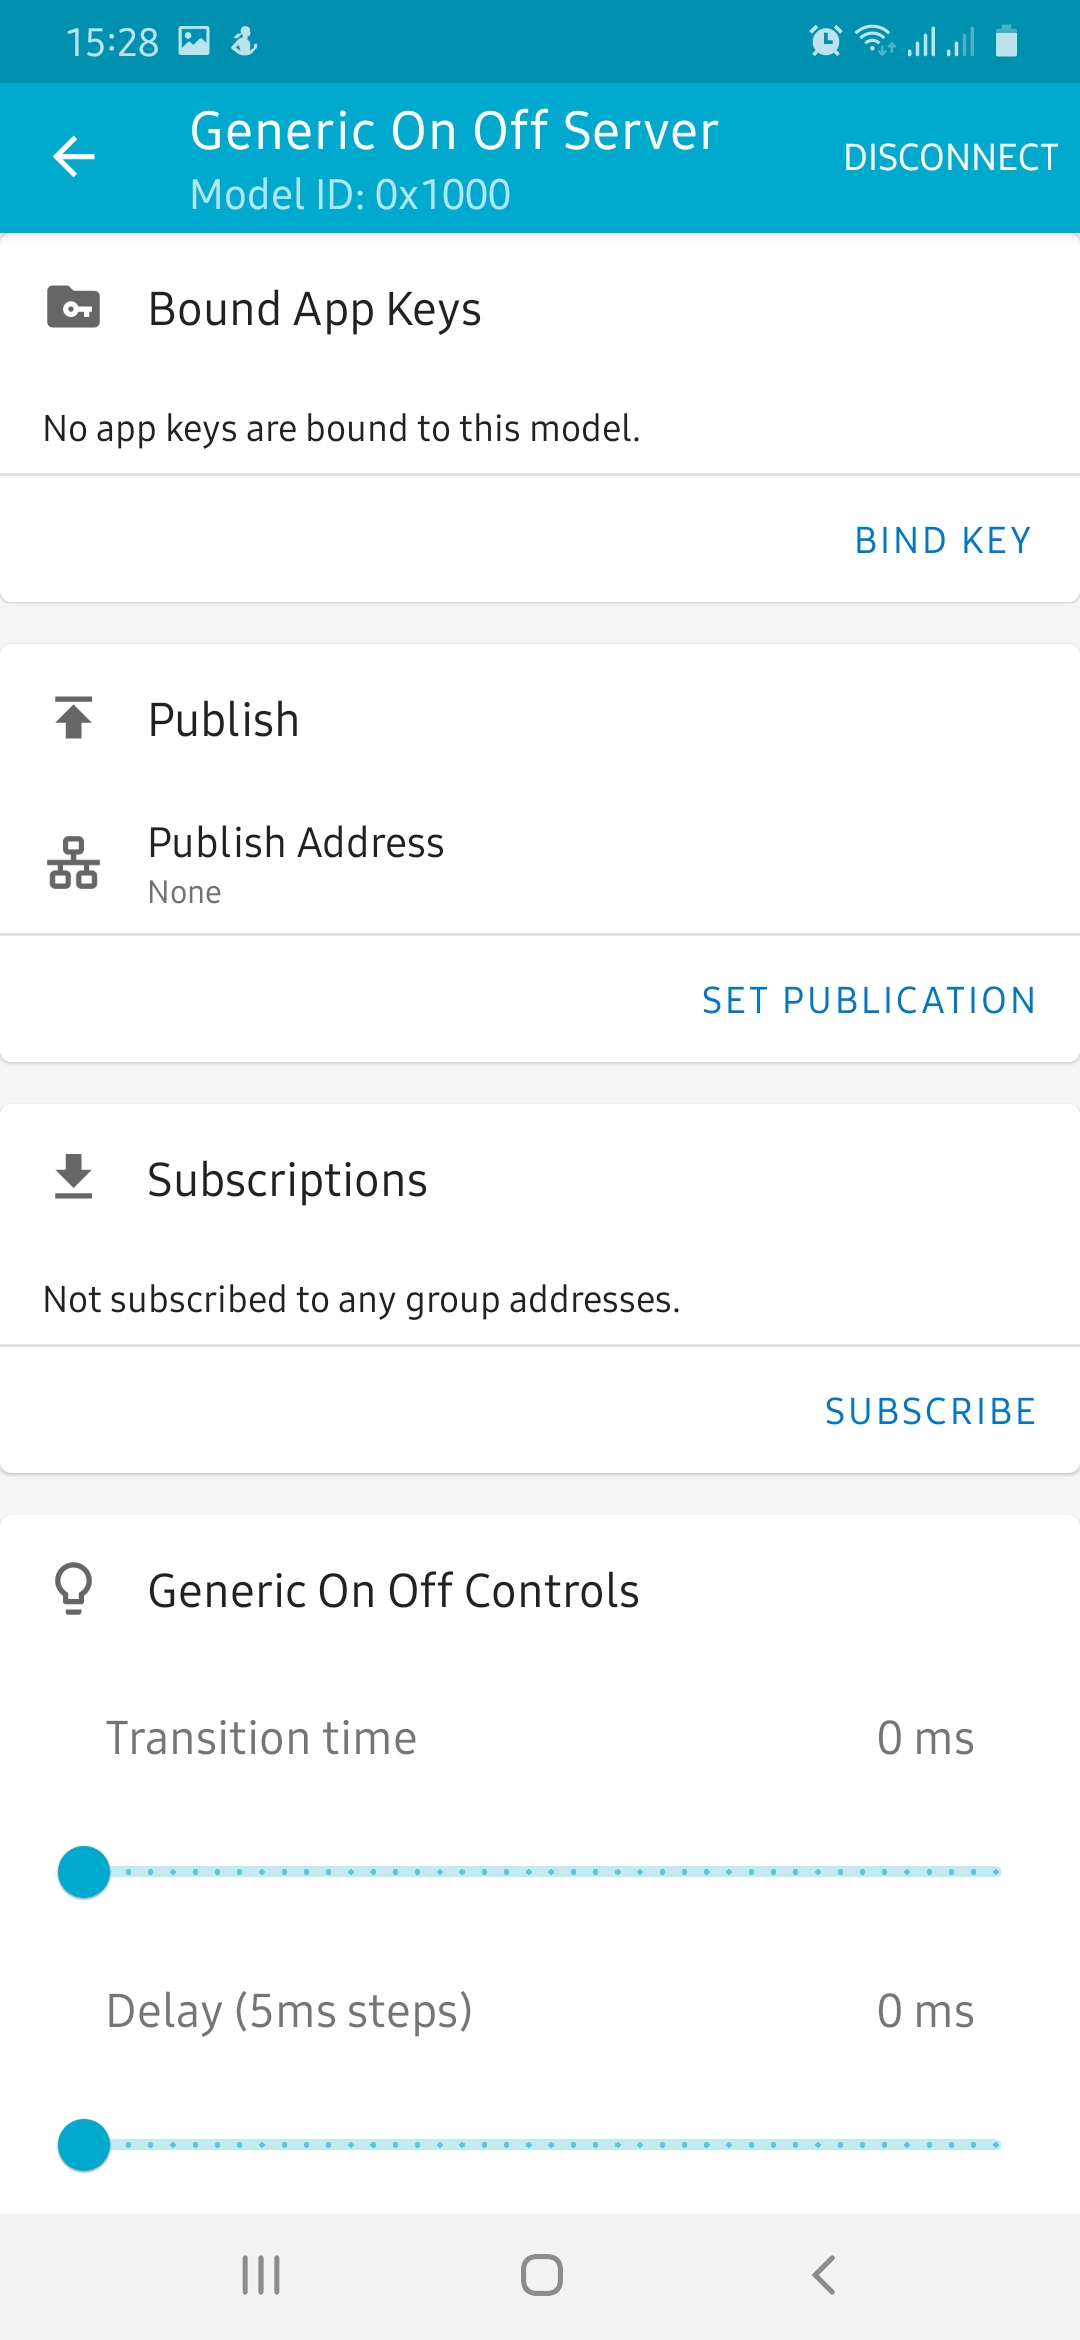
\includegraphics[width=0.7\linewidth]{nRF_Mesh_06.jpg}
        \caption{Element before configuration}
    \end{subfigure}
    \begin{subfigure}[b]{0.4\linewidth}
        \centering
        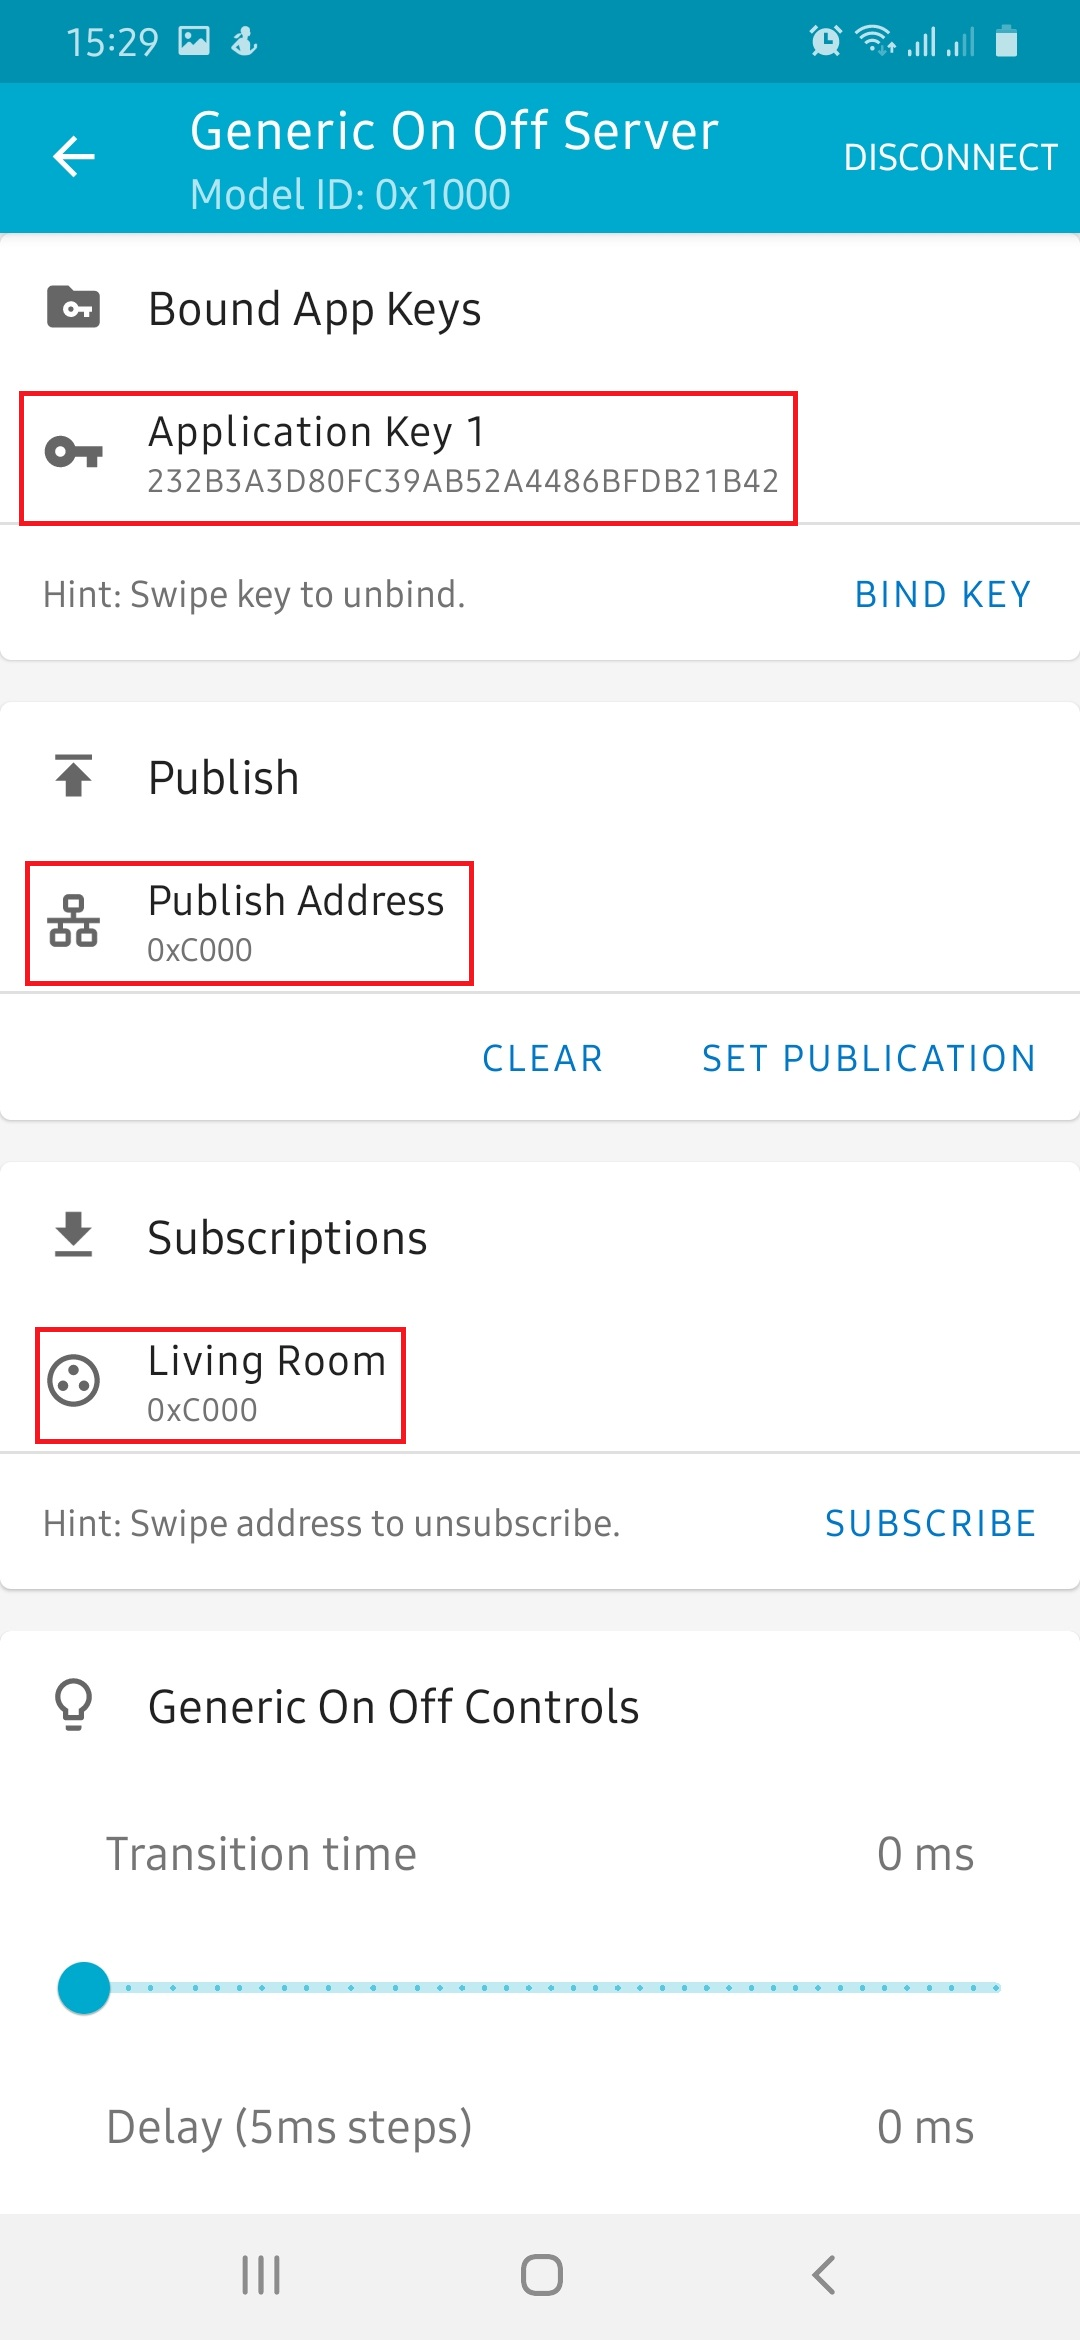
\includegraphics[width=0.7\linewidth]{nRF_Mesh_07.jpg}
        \caption{Element after configuration}
    \end{subfigure}
    \caption{Element configuration}
    \label{fig:element_configuration}
\end{figure}

\bib
\end{document}